\section{INTRODUCTION}
\begin{frame}{\secname}
\end{frame}

\subsection{The project}
\begin{frame}{\subsecname}
This project is based on the Kaggle challenge of the same name \cite{playground-series-s3e17}.

The data consisted in a set of various industrial devices, each described through attributes like torque or operating temperature, that did or did not suffer some kind of failure.

The task was therefore a binary classification between failed (class 1) and not-failed (class 0), which was done through several different models, from decision trees to a support vector machine.

All estimators (except for the first, as will be shown) were first run using default parameters, to achieve a baseline performance, then tuned with cross validation. All this was done using the \txt{scikit-learn} python package \cite{scikit-learn}, with the cross validation being performed using the \txt{GridSearchCV} and \txt{StratifiedKFold} classes.
\end{frame}

\subsection{Overview of the data}

\begin{frame}[label={attributes}]{\subsecname}
The attributes of each device are the following:
\begin{table}
    \centering
    \resizebox{\textwidth}{!}{
        \begin{tabular}{l|c|l}
            \textbf{Attribute} & \textbf{Datatype} & \textbf{Description} \\
            \hline\hline
            id & \txt{Int} & Device identifier  \\
            Product Id & \txt{String} & Unique Id, combination of the Type attribute and a number identifier \\
            Type & \txt{String} & Type of product/device (possible values: "L","M","H") \\       
            Air Temperature & \txt{Float} & Air temperature (Kelvin) \\
            Process Temperature & \txt{Float} & Production process temperature (Kelvin) \\
            Rotational Speed & \txt{Int} & Speed in RPM \\
            Torque & \txt{Float} & Torque in Nm (Newton Meter) \\
            Tool Wear & \txt{Int} & Time unit needed to wear down the product/tool \\
            TWF & \txt{Int} & Tool Wear Failure (binary) \\
            HDF & \txt{Int} & Heat Dissipation Failure (binary) \\
            PWF & \txt{Int} & Power Failure (binary) \\
            OSF & \txt{Int} & Overstrain Failure (binary) \\
            RNF & \txt{Int} & Random Failure (binary) \\
            \textbf{Machine Failure} & \txt{Int} & Failure binary feature (\textit{class attribute})
        \end{tabular}
    }
\end{table}
The fraction of devices belonging to each class is 98.43\% for class 0 and 1.57\% for class 1, a ratio of around 62 to 1.
\end{frame}

\begin{frame}{\subsecname}

\begin{figure}
    \centering
    \begin{subfigure}[c]{0.5\textwidth}
        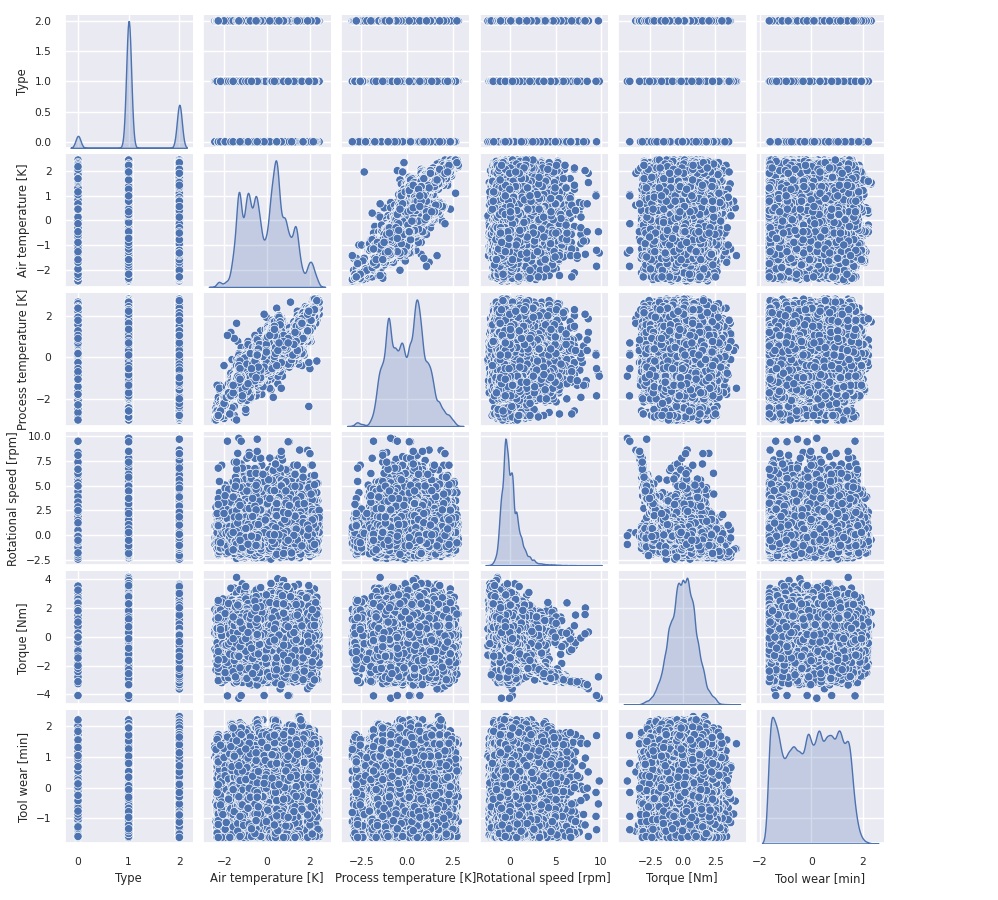
\includegraphics[width=\linewidth]{images/pairplot0.png}
        \caption{Class 0 pairplot}
        \label{fig:pairplot_0}
    \end{subfigure}\hfill
    \begin{subfigure}[c]{0.5\textwidth}
        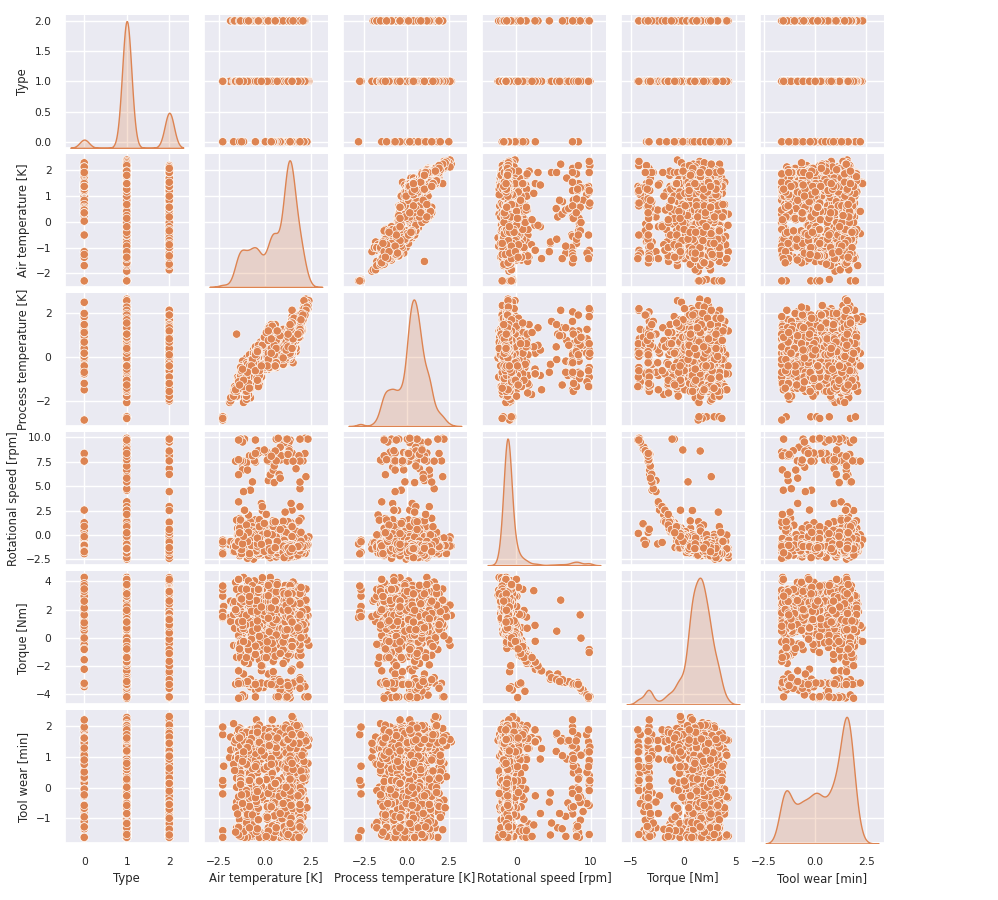
\includegraphics[width=\linewidth]{images/pariplot1.png}
        \caption{Class 1 pairplot}
        \label{fig:pairplot_1}
    \end{subfigure}
    \caption{Feature distributions per class (after preprocessing)}
    \label{fig:pairplots}
\end{figure}
\end{frame}

\subsection{Challenges}
\begin{frame}{\subsecname}
The main issue with the data is its extreme \textit{imbalance} between majority and minority class (see slide \ref{attributes}). This is addressed (mostly) by:
\begin{enumerate}
    \justifying
    \small
    \item resampling the minority class 
    \item choosing an appropriate metric for tuning
\end{enumerate}

Secondly, the dataset was actually generated from another one, leading to a few rows (822 out of around 132k) being clearly invalid and getting removed (their data couldn't be considered "reliable"). Specifically, these had a class inconsistent with their binary failure point (e.g., "Machine Failure" set to 0 but "HDF" set to 1).
\end{frame}

\subsection{Preprocessing and Resampling}
\begin{frame}{\subsecname}
The preprocessing simply comprised:
\begin{itemize}
    \small
    \justifying
    \item Removing the aforementioned incoherent rows, together with the TWF, HDF, PWF, OSF, RNF attributes (which would just be a copy of the class attribute)
    \item Removing the Product ID attribute, not relevant to the classification
    \item Normalizing all remaining features (except for Type, which is categorical)
\end{itemize}

The resampling specifically consisted in \textit{oversampling} the minority class to reach a minority-majority ratio of 1 to 10. This was done using the \mintinline{text}{imbalanced-learn} Python package \cite{imblearn}, which offers an implementation of the SMOTE oversampling method \cite{DBLP:journals/corr/abs-1106-1813}. Undersampling the majority was instead discarded because, in this case, it would mean removing a large number of rows to achieve the same ratio.

\end{frame}